\documentclass[parskip=full,11pt]{scrartcl}
%\usepackage{pdfpages}
\usepackage[utf8]{inputenc}
\usepackage{amssymb}
\usepackage[T1]{fontenc}
\usepackage[german]{babel}
\usepackage[yyyymmdd]{datetime} 
\usepackage{hyperref}
\usepackage[toc, nonumberlist, automake]{} %added automake option
\usepackage{csquotes}
\usepackage{graphicx}
\hypersetup{
 		pdftitle={Implementierung},
 }
\usepackage{fancyhdr}%<-------------to control headers and footers
\usepackage[a4paper,margin=1in,footskip=.25in]{geometry}
\fancyhf{}
\fancyfoot[C]{\thepage} %<----to get page number below text
\pagestyle{fancy} %<-------the page style itself
 
\title{Implementierung}
\subtitle{Autorisierungsmanagement für eine virtuelle Forschungsumgebung für Geodaten}
\author{Alex\\Anastasia\\Atanas\\Dannie\\ Houra\\Sonya\\}
\date{11.01.18}
 % define custom lists
\usepackage{enumitem}


\usepackage{linegoal,listings}
\newsavebox{\mylisting}
\makeatletter
\newcommand{\lstInline}[2][,]{%
	\begingroup%
	\lstset{#1}% Set any keys locally
	\begin{lrbox}{\mylisting}\lstinline!#2!\end{lrbox}% Store listing in \mylisting
	\setlength{\@tempdima}{\linegoal}% Space left on line.
	\ifdim\wd\mylisting>\@tempdima\hfill\\\fi% Insert line break
	\lstinline!#2!% Reset listing
	\endgroup%
}
\makeatother
\setlength{\parindent}{0pt}% Just for this example

\lstset{basicstyle=\footnotesize\ttfamily,breaklines=true}
\lstset{framextopmargin=50pt,frame=bottomline,showstringspaces=false,upquote=true}


 
\begin{document}
 
 \begin{titlepage}
 	
 	\begin{center}
 	
\includegraphics[width=0.5\linewidth]{res/KITLogo.png}\\
 	\vspace{2cm}
 	{\scshape\LARGE\bfseries Implementierung \par}
 	\vspace{0.5cm}
 	{\scshape\Large Praxis der Softwareentwicklung\\}
 	\vspace{1cm}
 	{\scshape\Large Wintersemester 17/18\\}
 	\vspace{2cm}
 	{\huge\bfseries Autorisierungsmanagement für eine virtuelle Forschungsumgebung für Geodaten\par}
 	\vspace{2cm}
 	\vfill
 	{\bfseries {\Large Autoren}:\par}
 	{\Large Bachvarov, Aleksandar }\\
 	{\Large Dimitrov, Atanas }\\
 	{\Large Mortazavi Moshkenan, Houraalsadat }\\
 	{\Large Sakly, Khalil }\\
 	{\Large Slobodyanik, Anastasia }\\
 	{\Large Voneva, Sonya}\\
 	\vfill
 	{\large 07.02.18 \par}
 	\end{center}
 \end{titlepage}
 
 \tableofcontents
 \newpage
 \section{Einleitung}
Dieses Dokument beschreibt die Änderungen, welche an unserem Entwurfdokument vorgenommen wurden, um die Funktionalität des Projekts ``Autorisierungsmanagement für eine virtuelle Forschungsumgebung für Geodaten`` zu gewährleisten. Das Ziel dieses Dokuments ist, die Gründe für diese Änderungen zu erläutern, beziehungsweise Probleme aufzuzeigen, die sich während der Implementierung ergeben haben.\\\\
Es werden Änderungen an Datenhaltung und Applikationslogik beschrieben sowie begründet. Des Weiteren wird ein Überblick darüber vermittelt, welche Musskriterien implementiert wurden, welche nicht und warum. Die implementierten Wunschkriterien werden ebenfalls kurz genannt.\\\\
Am Schluss des Dokuments befindet sich ein Vergleich zwischen unserem ursprünglichen und tatsächlichen Implementierungsplan sowie Erläuterungen eventueller Verzögerungen im Zeitplan.

 \newpage
 \section{Änderungen am Entwurf}
 
 \subsection{Model}
Während der Designphase wurden Klassen des Model-Pakets entsprechend der Prinzipien objektorientierter Programmierung entworfen. Während der Einarbeitung in das Django-Framework hat sich allerdings herausgestellt, dass Model-Klassen eher als Datenstruktur-Träger benutzt werden und keine Anwendungslogik in sich kapseln. Daher wurde sämtliche Funktionalität in dem View-Paket implementiert, sodass Model-Klassen ausschließlich die Datenbankstruktur definieren.
 
\begin{itemize}
\item \textbf{Klasse CustomUser}\\
Klasse \textit{CustomUser} erbt von der Django-Klasse \textit{User} und ersetzt Klasse \textit{User} aus dem Entwurfdokument. Sämtliche Attribute werden von Django vordefiniert und mussten nicht zusätzlich implementiert werden.

\item \textbf{Klasse Admin}\\
Da diese Klasse keine Funktionalität in sich kapselt, hat sich herausgestellt, dass sie durch die Benutzung des Attributs \textit{is staff} ersetzt werden kann. Dieses Attribut wird in der \textit{User}-Klasse von Django vordefiniert.
 
\item\textbf{Klasse Resource}\\
Um Lese- und Besitzerrechte zu implementieren, werden der Klasse zusätzliche Attribute hinzugefügt: die Listen \textit{Readers} und \textit{Owners}.

\item \textbf{Klasse ResourceType}\\
TO DO

\item \textbf{Klasse Request}\\
Dieser Klasse wurde das \textit{Description}-Attribut hinzugefügt. Dieses Attribut hat Type \textit{String} und dient dazu, die Begründung zu speichern, welche vom Absender bei der Erstellung des Requests eventuell eingegeben wurde.

\item \textbf{Klassen Logging und EmailMessages}\\
Diese von Django vordefinierten Klassen mussten nicht extra implementiert werden. 
\end{itemize}

\newpage
\subsection{View} 
 
\begin{itemize}
\item \textbf{Klasse ChosenRequestsView}\\
Funktionalität dieser Klasse wurde auf vier Views verteilt:
\begin{itemize}
\item \textit{ApproveAccessRequest}
\item \textit{DenyAccessRequest}
\item \textit{ApproveDeletionRequest}
\item \textit{DenyDeletionRequest}
\end{itemize}
Diese Unterteilung hat bessere Trennung der Anwendungslogik für Bearbeitung unterschiedlicher Requests zur Folge. 

\item \textbf{Klasse DeleteResourceView}\\
Dieser View erweitert Funktionalität von Klassen \textit{ManageResourcesView} und \textit{ResourcesOverview} und wird zum Löschen der Ressourcen von Administratoren des Portals benutzt. Absenden eines Löschrequests wird stattdessen im \textit{SendDeletionRequestView} implementiert. 

\item \textbf{Klassen PermissionForChosenResourceView,  PermissionsForResourceView und PermissionsForUsersView}\\
Diese Views wurden durch \textit{PermissionEditingView} ersetzt und für bessere Übersichtlichkeit durch  \textit{PermissionEditingViewSearch} erweitert. Bearbeitung der Rechte aller Ressourcen in einem View hat bessere Benutzbarkeit des Portals zur Folge.

\item \textbf{Klassen ManageUsersView und ManageResourcesView}\\
Diese Views wurden durch vordefinierte Django-Funktionalität ersetzt.

\item \textbf{Klasse ResourcesOverview}\\
Dieser View wurde durch einen zusätzlichen View \textit{ResourcesOverviewSearch} für bessere Benutzbarkeit des Portals erweitert.

\item \textbf{Klasse RequestView}\\
Funktionalität dieses Views wurde für bessere Struktur der Anwendungslogik auf vier Views verteilt:
\begin{itemize}
\item \textit{SendAccessRequest}
\item \textit{CancelAccessRequest}
\item \textit{ApproveDeletionRequest}
\item \textit{DenyDeletionRequest}
\end{itemize}

\item \textbf{Klasse ResourceInfoView}\\
Funktionalität dieses Views wurde durch einen Modaldialog implementiert, um überflüssige Codezeilen zu sparen.
\newpage
\item \textbf{Zusätzlich implementierte Views}\\
Während der Implementierung hat sich herausgestellt, dass einige Funktionalitäten des Portals zusätzliche View-Klassen benötigen. Die noch nicht erwähnten Views heißen:
\begin{itemize}
\item \textit{AddNewResourceView} dient zur Erstellung einer neuen Ressource;
\item \textit{EditNameView} wird zum Ändern des Benutzernamens benutzt.
\end{itemize} 
\end{itemize}

\subsection{URL-Verzeichnis}
Änderungen an Views haben dementsprechende Änderungen am URL-Verzeichnis verursacht. Eine URL lokalisiert einen View, der entweder als ein Main-Fenster oder dessen Teil präsentiert wird.  \\
\renewcommand{\labelitemi}{$\bullet$}
\renewcommand{\labelitemii}{}
\renewcommand{\labelitemiii}{}
\renewcommand{\labelitemiv}{}  

\indent Home-Seite mit Authentifizierungsfunktionalität für Testzwecke:
\begin{itemize}[itemsep=0pt]
\item \textbf{/home}
	\begin{itemize}[itemsep=0pt]
	\item \textbf{/register}
	\item \textbf{/login}
	\item \textbf{/logout}\\
	\end{itemize}

\noindent Verwaltungsseiten:
\item \textbf{/resource-manager}
\item \textbf{/user-manager}\\

\noindent Benutzerseite:
\item \textbf{/profile}
	\begin{itemize}[itemsep=0pt]
	\item \textbf{/my-resources}
		\begin{itemize}
		\item \textbf{/resourceid-edit-users-permissions}
			\begin{itemize}
			\item \textbf{/search}
			\end{itemize}
		\item \textbf{/add-new-resource}		
		\end{itemize}
	\item \textbf{/edit-name}\\
	\end{itemize}

\noindent Bearbeitung der Requests:
\item \textbf{/approve-access-request/requestid}
\item \textbf{/deny-access-request/requestid}
\item \textbf{/approve-deletion-request/requestid}
\item \textbf{/deny-deletion-request/requestid}\\

\noindent Absenden und Löschen der Requests:
\item \textbf{/send-access-request/resourceid}
\item \textbf{/cancel-access-request/resourceid}
\item \textbf{/send-deletion-request/resourceid}
\item \textbf{/cancel-deletion-request/resourceid}\\

\noindent Ressourcenübersicht:
\item \textbf{/resources-overview}
	\begin{itemize}
	\item \textbf{/search}\\
	\end{itemize}
	
\noindent Metadaten einer Ressource
\item \textbf{/resources/resourceid}\\

\noindent Löschen der Ressourcen für Administratoren:
\item \textbf{/delete-resource/resourceid}
\end{itemize}
 
\newpage 
\subsection{Datenbank}
Jede Änderung am Model-Paket beeinflusst Datenbankstruktur. Das von Django unabhängiges Teil der Datenbank, die für die Datenhaltung in unserem Projekt benutzt wird, wird auf der Abbildung 1 dargestellt. Die im Entwurf geplante Tabelle \textit{Permission} wurde durch \textbf{many-to-many} Beziehungen zwischen Benutzern und Ressourcen ersetzt und in zwei Tabellen \textit{Resource Owners} und \textit{Resource Readers} zu speichern. Diese Änderung sorgt für bessere Antwortzeit der Datenbank, was wiederum zur besseren Benutzbarkeit dient.
Unterschiedliche Arten von Requests werden in getrennten Tabellen gespeichert. Das ermöglicht bessere Trennung zwischen Benutzer- und Admin-Funktionalitäten. Bearbeitete Requests werden nicht weiter gespeichert und sind ausschließlich in der Logdatei zum nachverfolgen.    
 \begin{figure}[ht!]
 	\centering
 	\includegraphics[width=0.9\textwidth]{res/database.png}
 	\caption{Schema der Datenbank. Jedes Rechteck repräsentiert eine Tabelle,
jedes Attribut - eine Spalte in der entsprechenden Tabelle in der Datenbank. Die
Pfeile geben Auskunft welches Attribut in welcher Tabelle als Schlüssel vorkommt.}
 \end{figure}

\newpage
\section{Implementierte Kriterien}
\subsection{Musskriterien}
Während der Planungsphase wurde eine Anforderungsdefinition im Pflichtenheft festgelegt. Diese Anforderungen beschreiben welche Muss-, Wunsch- und Abgrenzungskriterien das zu entwickelnde Produkt erfüllen muss. In der Implementierungsphase unseres Projekts wurden alle Musskriterien erfolgreich implementiert, was an präzise und eindeutige Aufgabeformulierung verweist und zeigt, dass das Wasserfallmodel an Softwareentwicklung ergebnisreich angewendet werden kann.   

\subsection{Wunschkriterien}
Bei der Implementierung funktionaler Anforderungen hat sich ergeben, dass Realisierung einiger Wunschkriterien die Benutzbarkeit des Produkts deutlich verbessern würde. Als Folge wurden unten genannte Kriterien zusätzlich implementiert:
\begin{itemize}
\item Wird eine Ressource gelöscht, so werden alle Besitzer per E-Mail benachrichtigt.
\item Ein Benutzer kann durch Administratoren blockiert werden.
\item Der Administrator kann Benutzer anhand von Vorname und/oder Nachname suchen.
\end{itemize}


\newpage
\section*{Unittests}
\subsection*{Setup}
\begin{itemize}
\item \textbf{setUpUsers}
\item \textbf{setUpResourceAndRequests}
\end{itemize}
\subsection*{Test Cases}
\begin{itemize}
\item \textbf{TestHomeView}
\item \textbf{TestResourceManager}
\item \textbf{TestUserManager}
\item \textbf{TestProfileView}
\item \textbf{TestMyResourcesView}
\item \textbf{TestResourcesOverview}
\item \textbf{TestResourcesOverviewSearch}
\item \textbf{TestPermissionEditingView}
\item \textbf{TestPermissionEditingViewSearch}

\end{itemize}
\subsection*{Cleanup}
\begin{itemize}
\item \textbf{deleteUsers}
\item \textbf{deleteResourcesAndRequests}
\end{itemize}

\newpage
\section{Implementierungsplan}
Am Anfang wurde Zeitplan erstellt (Abbildung 2). Aufwandsschätzung benutzt. Keine Erfahrung mit Django - Abweichungen als Folge.\\\\
Änderungen an einem Teil verursachen Änderungen an schon implementierten Modulen - Task wird neu aufgemacht - Zeit verdoppelt sich. Schwere Planung wegen Abhängigkeiten der Modulen - Versagen des Wasserfallmodels. Trennung der Aufgaben meist schwer und unrealistisch.\\\\ 
Realer Zeitablauf (Abbildung 3) zeigt Verzögerungen bei geplanten Aktivitäten und Maas der Auswirkung jeder Verzögerung auf gesamten Zeitverlauf. 
Trotz allen Ungeschicklichkeiten nur 3 Tage Verspätung bei der Abgabe.\\


 \begin{figure}[ht!]
 	\centering
 	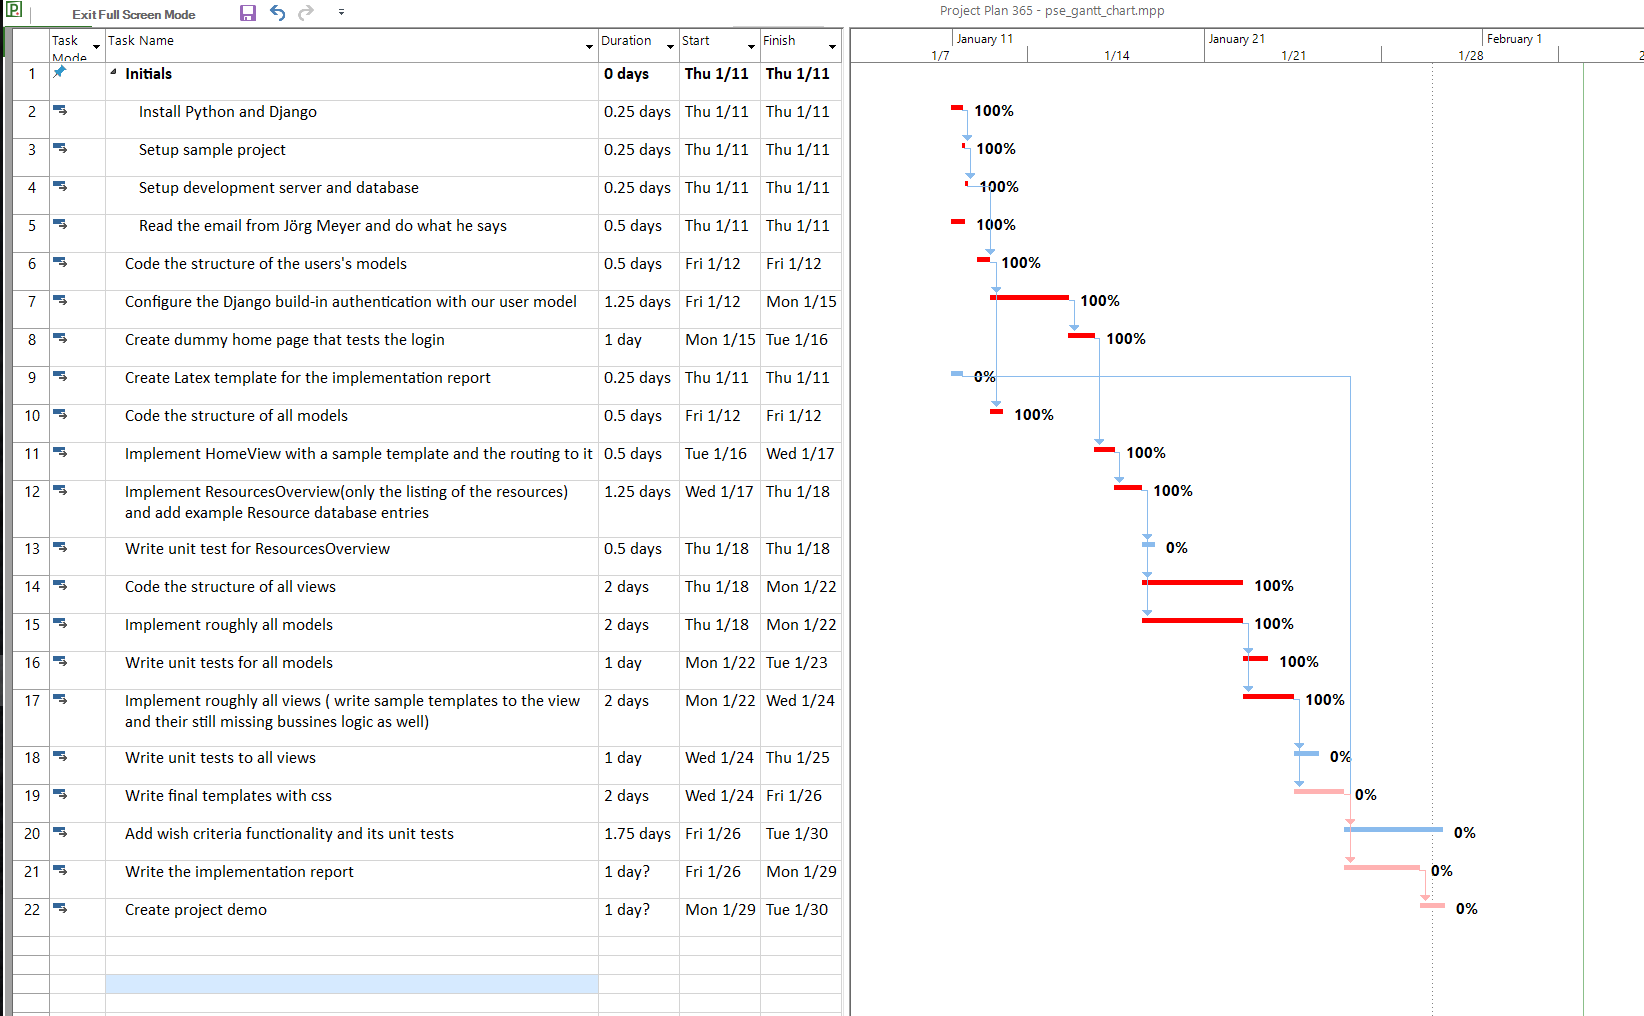
\includegraphics[width=0.9\textwidth]{res/gannt_plan.png}
 	\caption{Ursprünglicher Implementierungsplan. Jede Aktivität wird in jeweiliger Zeile mit einem waagerechten Balken visualisiert. Je länger der Balken, desto länger dauert die Aktivität. Die Beziehungen (beziehungsweise Abhängigkeiten) zwischen Aktivitäten werden mit Pfeilen dargestellt.}
 \end{figure}
  \begin{figure}[ht!]
 	\centering
 	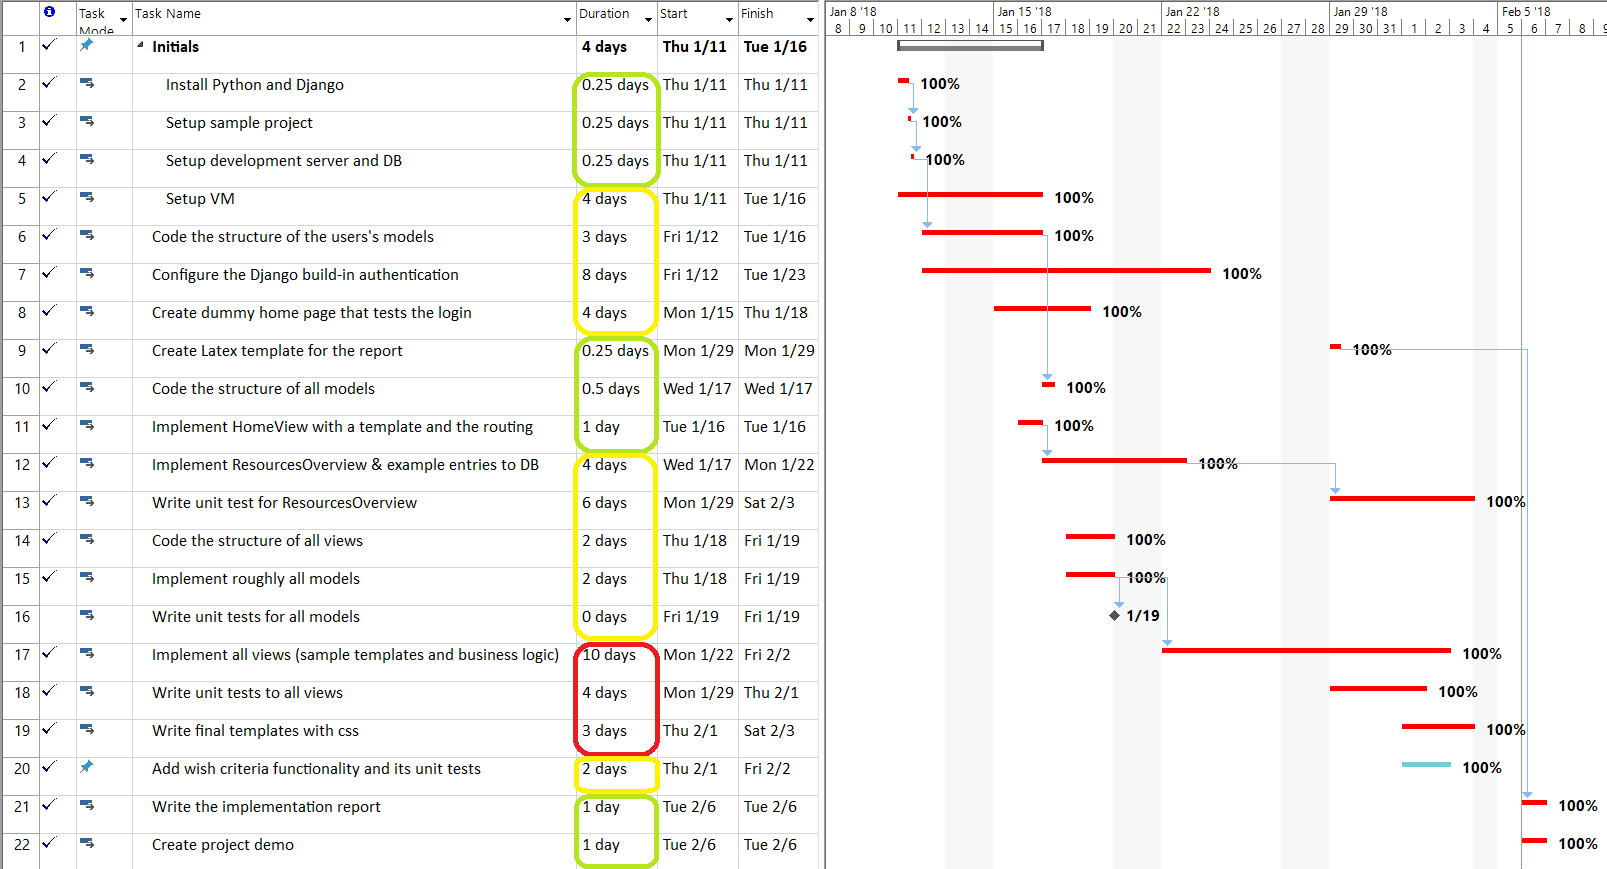
\includegraphics[width=0.9\textwidth]{res/gannt_real.png}
 	\caption{Realer Zeitablauf der Implementierung mit geänderter Dauer der Aktivitäten. Abhängig von Folgen der Verzögerungen werden Aktivitäten farblich markiert: grün - rechtzeitig/keine negative Folgen, gelb - von anderen Aktivitäten verursachte Verzögerungen, rot - Aktivitäten, während deren Entwurfsprobleme gelöst werden mussten}
 \end{figure}
\end{document}
\grid
